\documentclass[9pt,aspectratio=169,xcolor=table]{beamer}

%~~~~~~~~~~~~~~~~~~~~~~~~~~~~~~~~~~~~~~~~~~~~~~~~~~~~~~~~~~~~~~~~~~~~~~~~~~~~~~
% Use roboto Font (recommended)
\usepackage[sfdefault]{roboto}
\usepackage[utf8]{inputenc}
\usepackage[T1]{fontenc}
%~~~~~~~~~~~~~~~~~~~~~~~~~~~~~~~~~~~~~~~~~~~~~~~~~~~~~~~~~~~~~~~~~~~~~~~~~~~~~~

%~~~~~~~~~~~~~~~~~~~~~~~~~~~~~~~~~~~~~~~~~~~~~~~~~~~~~~~~~~~~~~~~~~~~~~~~~~~~~~
% Define where theme files are located. ('/styles')
\usepackage{styles/fluxmacros}
\usefolder{styles}
% Use Flux theme v0.1 beta
% Available style: asphalt, blue, red, green, gray
% "red" is the closest built-in style to maroon; its exact colours are
% overridden with a true maroon palette just below, after the theme loads.
\usetheme[style=red]{flux}
%~~~~~~~~~~~~~~~~~~~~~~~~~~~~~~~~~~~~~~~~~~~~~~~~~~~~~~~~~~~~~~~~~~~~~~~~~~~~~~

%~~~~~~~~~~~~~~~~~~~~~~~~~~~~~~~~~~~~~~~~~~~~~~~~~~~~~~~~~~~~~~~~~~~~~~~~~~~~~~
% SKEE1033 maroon palette override.
% The flux theme's colortheme defines primaryLight/primary/secondary/tertiary
% as plain \definecolor calls (not \providecolor), so simply redefining them
% here, AFTER \usetheme, wins -- xcolor allows redefinition and every
% \setbeamercolor in beamercolorthemeflux.sty was already evaluated against
% these names, so the redefinition propagates everywhere automatically.
\definecolor{primaryLight}{HTML}{9B2242} % lighter maroon -- headers, accents
\definecolor{primary}{HTML}{7B1E3A}      % core maroon -- titles, block headers
\definecolor{secondary}{HTML}{3A5A6B}    % muted teal -- complementary accent
\definecolor{tertiary}{HTML}{8C6A3F}     % warm bronze -- example/third accent
%~~~~~~~~~~~~~~~~~~~~~~~~~~~~~~~~~~~~~~~~~~~~~~~~~~~~~~~~~~~~~~~~~~~~~~~~~~~~~~

%~~~~~~~~~~~~~~~~~~~~~~~~~~~~~~~~~~~~~~~~~~~~~~~~~~~~~~~~~~~~~~~~~~~~~~~~~~~~~~
% Extra packages
\usepackage{booktabs}
\usepackage{colortbl}
\usepackage{ragged2e}
\usepackage{amssymb}
\usepackage{multirow}
\usepackage{tikz}
\usetikzlibrary{arrows.meta, positioning, fit, backgrounds, calc, shapes.geometric}
\setbeamertemplate{itemize items}[square]
\usepackage[scaled=.92]{beramono}
\usepackage{listings}
\usepackage{array}
% Table striping: odd rows white, even rows very light gray.
\definecolor{stripe}{gray}{0.94}
\newcommand{\striped}{\rowcolors{1}{white}{stripe}}
%~~~~~~~~~~~~~~~~~~~~~~~~~~~~~~~~~~~~~~~~~~~~~~~~~~~~~~~~~~~~~~~~~~~~~~~~~~~~~~

%~~~~~~~~~~~~~~~~~~~~~~~~~~~~~~~~~~~~~~~~~~~~~~~~~~~~~~~~~~~~~~~~~~~~~~~~~~~~~~
% Code listing style (lightweight analogue of the book's skpython style).
% This course is Python-only, so Python is set as the lstlisting default via
% \lstset below -- every \begin{lstlisting} needs no language=... of its own.
% The one exception is the pseudocode frame later in this deck, which opts
% out explicitly with language={} since it is not real Python.
\definecolor{codebg}{HTML}{FBF2F4}
\definecolor{codegreen}{rgb}{0,0.45,0}
\definecolor{codestring}{rgb}{0.58,0.1,0.2}
\lstdefinestyle{skpython}{
    basicstyle=\ttfamily\footnotesize,
    keywordstyle=\color{primary}\bfseries,
    commentstyle=\itshape\color{codegreen},
    stringstyle=\ttfamily\color{codestring},
    backgroundcolor=\color{codebg},
    breaklines=true,
    keepspaces=true,
    showspaces=false,
    showstringspaces=false,
    frame=single,
    rulecolor=\color{primary!40},
    numbers=none,
}
\lstset{language=Python, style=skpython}
%~~~~~~~~~~~~~~~~~~~~~~~~~~~~~~~~~~~~~~~~~~~~~~~~~~~~~~~~~~~~~~~~~~~~~~~~~~~~~~

%~~~~~~~~~~~~~~~~~~~~~~~~~~~~~~~~~~~~~~~~~~~~~~~~~~~~~~~~~~~~~~~~~~~~~~~~~~~~~~
% TikZ block styles for the computation-cycle and control-structure diagrams
\definecolor{cycfill}{HTML}{F3DCE4}
\definecolor{cycline}{HTML}{7B1E3A}
\definecolor{cycdofill}{HTML}{E8EEF0}
\definecolor{cycdoline}{HTML}{3A5A6B}
\tikzset{
  cycstep/.style = {font=\sffamily\small, align=center, rounded corners=2pt,
                     draw=cycline, fill=cycfill, line width=0.7pt,
                     minimum height=7mm, minimum width=20mm, inner sep=3pt},
  cycdo/.style   = {cycstep, fill=cycdofill, draw=cycdoline},
  flow/.style    = {-{Stealth[length=2mm]}, thick, draw=cycline},
}
%~~~~~~~~~~~~~~~~~~~~~~~~~~~~~~~~~~~~~~~~~~~~~~~~~~~~~~~~~~~~~~~~~~~~~~~~~~~~~~

%%%%%%%%%%%%%%%%%%%%%%%%%%%%%%%%%%%
%% SECTION SEPARATOR (ToC recap) %%
%%%%%%%%%%%%%%%%%%%%%%%%%%%%%%%%%%%
\AtBeginSection[]
{
{
    \setbeamercolor{background canvas}{bg=primaryLight!6}
    \begin{frame}[plain]
        \frametitle{Table of Contents}
        \tableofcontents[currentsection]
    \end{frame}
}
}
%%%%%%%%%%%%%%%%%%%%%%%%%%%%%%%%%%%

%~~~~~~~~~~~~~~~~~~~~~~~~~~~~~~~~~~~~~~~~~~~~~~~~~~~~~~~~~~~~~~~~~~~~~~~~~~~~~~
% Information
\title{Computing as an Engineering Tool}
\subtitle{\emph{Engineering Computation with Python} --- Chapter 1}
\author{Mun\'{i}m Zabidi}
\institute{\color{primary}Faculty of Electrical Engineering, Universiti Teknologi Malaysia}
\date{\today}
\titlegraphic{assets/logoutmwhite.png}
%~~~~~~~~~~~~~~~~~~~~~~~~~~~~~~~~~~~~~~~~~~~~~~~~~~~~~~~~~~~~~~~~~~~~~~~~~~~~~~

\begin{document}

\titlepage

\begin{frame}{Table of Contents}
    \tableofcontents
\end{frame}

%===============================================================================
\section{Why Engineers Compute}
%===============================================================================

\begin{frame}{Why Does an Engineer Need to Compute at All?}
    \leavevmode
    Consider one of the first equations you meet in electrical engineering,
    Ohm's law:
    \[
    V = IR, \qquad\text{or equivalently}\qquad I = \frac{V}{R}.
    \]

    \vspace{2mm}
    A $12\,\text{V}$ supply is connected across a $470\,\Omega$ resistor.
    You need the current. There are three ways to get it.

    \vspace{3mm}
    \begin{columns}[t]
        \begin{column}{.33\textwidth}
            \begin{block}{By hand}
                \small
                $I = \dfrac{12}{470} \approx 25.5\,\text{mA}$

                \vspace{1mm}
                Fast for one resistor. Leaves no record.
            \end{block}
        \end{column}
        \begin{column}{.33\textwidth}
            \begin{block}{With a calculator}
                \small
                Key in $12 \div 470$.

                \vspace{1mm}
                Faster still. Nobody --- including you, next week --- can
                check what you did.
            \end{block}
        \end{column}
        \begin{column}{.33\textwidth}
            \begin{block}{With Python}
                \small
                \texttt{I = V / R}

                \vspace{1mm}
                Looks like more work \ldots for one resistor.
            \end{block}
        \end{column}
    \end{columns}
\end{frame}

\begin{frame}[fragile]{The Question That Changes Everything}
    \leavevmode
    \begin{center}
    \fbox{\parbox{.8\textwidth}{\centering\vspace{2mm}
    \large What if there are 10\,000 measurements?
    \vspace{2mm}}}
    \end{center}

    \vspace{4mm}
    A data logger records voltage once per second for nearly three hours.
    You need the current at every instant, the average power, the maximum
    current, and a plot.

    \vspace{2mm}
    \begin{itemize}
        \item By hand: impossible.
        \item With a calculator: impossible.
        \item With Python: a few lines --- and the \alert{same} few lines
              work for ten measurements or ten million.
    \end{itemize}

    \vspace{3mm}
    \begin{block}{The point}
        Programming is not a separate skill added on top of engineering;
        it is what makes engineering calculations \alert{scale} from the
        textbook to the laboratory.
    \end{block}
\end{frame}

\begin{frame}{The Engineering Computation Cycle}
    \leavevmode
    Every worked example in this course, from this slide to the final
    chapter, follows the same cycle:

    \begin{center}
    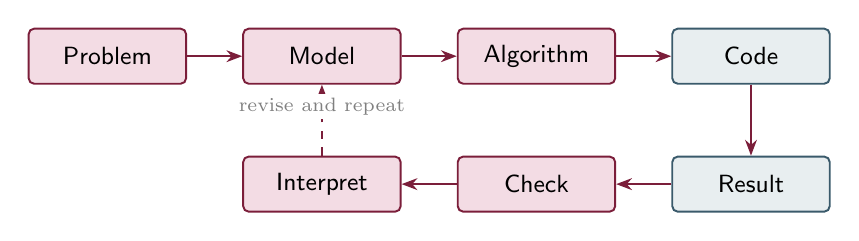
\begin{tikzpicture}[node distance=5mm and 7mm]
        \node[cycstep]                    (prob) {Problem};
        \node[cycstep, right=of prob]     (mod)  {Model};
        \node[cycstep, right=of mod]      (alg)  {Algorithm};
        \node[cycdo,   right=of alg]      (code) {Code};
        \node[cycdo,   below=9mm of code] (res)  {Result};
        \node[cycstep, left=of res]       (chk)  {Check};
        \node[cycstep, left=of chk]       (intp) {Interpret};
        \draw[flow] (prob) -- (mod);
        \draw[flow] (mod)  -- (alg);
        \draw[flow] (alg)  -- (code);
        \draw[flow] (code) -- (res);
        \draw[flow] (res)  -- (chk);
        \draw[flow] (chk)  -- (intp);
        \draw[flow, dashed] (intp.north) -- node[font=\scriptsize, text=Gray, fill=white, inner sep=1.5pt, above, pos=0.5]
              {revise and repeat} (mod.south);
    \end{tikzpicture}
    \end{center}

    \vspace{2mm}
    \begin{alertblock}{The two steps engineers most often skip}
        \textbf{Check} and \textbf{Interpret}. A computer executes wrong
        instructions just as precisely as right ones --- a result that has
        not been checked is not yet an answer.
    \end{alertblock}
\end{frame}

\begin{frame}[fragile]{A First Engineering Calculation}
    \leavevmode
    An LED needs a series resistor to limit its current. Supply
    $5\,\text{V}$, LED drop $2\,\text{V}$, desired current $20\,\text{mA}$:
    \[
    R = \frac{V_{\text{supply}} - V_{\text{LED}}}{I}.
    \]

    \begin{columns}[t]
        \begin{column}{.55\textwidth}
\begin{lstlisting}
V_supply = 5.0   # volts
V_led    = 2.0   # volts
I_led    = 0.02  # amps

R = (V_supply - V_led) / I_led
print("R =", R, "ohms")
\end{lstlisting}
            \texttt{R = 150.0 ohms}
        \end{column}
        \begin{column}{.42\textwidth}
            \small
            \textbf{Check.} Volts $\div$ amps $=$ ohms. Magnitude is
            plausible for an LED series resistor.

            \vspace{2mm}
            \textbf{Interpret.} $150\,\Omega$ may not be a standard value
            --- fit the nearest available ($150\,\Omega$ or
            $220\,\Omega$) and accept a slightly different current.
        \end{column}
    \end{columns}
\end{frame}

\begin{frame}{The Bench Experiment Used Throughout This Course}
    \leavevmode
    \small
    One real measurement, returned to in every chapter, so each new
    technique applies to data you already understand.

    \vspace{2mm}
    \begin{columns}[t]
        \begin{column}{.5\textwidth}
            \textbf{The experiment.} A $100\,\mu\text{F}$ capacitor,
            charged to $12\,\text{V}$, discharges through a
            $4.7\,\text{k}\Omega$ resistor. Logged every $20\,\text{ms}$
            for two seconds: time, voltage, current, temperature.
            \[
            v(t) = V_0\,e^{-t/\tau}, \qquad \tau = RC = 0.47\,\text{s}.
            \]
        \end{column}
        \begin{column}{.5\textwidth}
            \textbf{Why one dataset.} A genuine recording, not a tidy
            formula --- it has noise, three dropped samples near
            $t=0.8\,\text{s}$, and one corrupted temperature reading.

            \vspace{2mm}
            These flaws are not accidents: they are why several later
            chapters exist (data quality, curve fitting, calculus).
        \end{column}
    \end{columns}
\end{frame}

%===============================================================================
\section{Programming Fundamentals}
%===============================================================================

\begin{frame}{What Is Programming?}
    \leavevmode
    We define a computer, simply, as \alert{one that computes}: a
    programmable electronic device that can store, retrieve, and process
    data.

    \vspace{3mm}
    Many everyday actions already follow a logical sequence of steps ---
    turning a page of a book, by hand:
    \begin{enumerate}\itemsep1pt
        \item Lift hand.
        \item Move hand to the right side of the book.
        \item Grasp the top-right corner of the page.
        \item Move the hand from right to left until positioned.
        \item Let go of the page.
    \end{enumerate}

    \vspace{2mm}
    \begin{block}{Definition}
        Describing the order and sequence of operations in a process is
        called \alert{programming}. The list of steps a computer follows
        is a \alert{program}.
    \end{block}
\end{frame}

\begin{frame}{The Three Phases of Program Development}
    \leavevmode
    \small
    \begin{columns}[t]
        \begin{column}{.33\textwidth}
            \begin{block}{Phase 1: Problem Solving}
                \scriptsize
                \begin{itemize}
                    \item Analysis and specification
                    \item General solution (algorithm)
                    \item Verify
                \end{itemize}
            \end{block}
        \end{column}
        \begin{column}{.33\textwidth}
            \begin{block}{Phase 2: Implementation}
                \scriptsize
                \begin{itemize}
                    \item Concrete solution (program)
                    \item Test
                \end{itemize}
            \end{block}
        \end{column}
        \begin{column}{.33\textwidth}
            \begin{block}{Phase 3: Maintenance}
                \scriptsize
                \begin{itemize}
                    \item Use
                    \item Maintain
                \end{itemize}
            \end{block}
        \end{column}
    \end{columns}

    \vspace{3mm}
    \begin{alertblock}{A program is rarely finished}
        These three phases form a cycle. A program is usually not
        complete just because it runs correctly once: requirements
        change, and new errors are discovered during real use.
    \end{alertblock}
\end{frame}

\begin{frame}{What Is an Algorithm?}
    \leavevmode
    A computer program and an algorithm look similar because
    \alert{all programs are algorithms} --- a program is simply an
    algorithm written in a form a computer can execute.

    \vspace{2mm}
    \begin{block}{Informal definition}
        An algorithm is a verbal or written description of a logical
        sequence of actions --- a recipe, a set of instructions, a set
        of directions.
    \end{block}

    \vspace{2mm}
    \textbf{Four equivalent ways to describe an algorithm:}
    \begin{enumerate}\itemsep1pt
        \item Step-by-step diagrams (e.g.\ origami instructions)
        \item \alert{Flowcharts} --- boxes and arrows
        \item A list of plain-language steps
        \item \alert{Pseudocode} --- resembles a real language, tied to none
    \end{enumerate}
\end{frame}

\begin{frame}{Example: Starting a Car}
    \leavevmode
    \small
    \begin{enumerate}\itemsep2pt
        \item Insert the key.
        \item Depress the brake pedal.
        \item Make sure the transmission is in Park (or neutral).
        \item Turn the key to the start position.
        \item If the engine starts within six seconds, release the key to
              the ignition position.
        \item If the engine doesn't start, release the key and the gas
              pedal, wait ten seconds, and repeat steps 3--6, but not
              more than five times.
        \item If the car still doesn't start, call the garage.
    \end{enumerate}

    \vspace{2mm}
    \begin{block}{Notice}
        Every step is unambiguous, and the sequence includes a
        \alert{decision} (step 5) and a \alert{repeat} (step 6) --- the
        two control structures beyond plain sequence.
    \end{block}
\end{frame}

\begin{frame}{The Four Control Structures}
    \leavevmode
    \small
    Regardless of language, every algorithm is built from just four
    control structures:

    \vspace{2mm}
    \begin{columns}[t]
        \begin{column}{.5\textwidth}
            \begin{block}{Sequence}
                \scriptsize Statements executed one after another.
                Nothing branches, nothing repeats.
            \end{block}
            \vspace{2mm}
            \begin{block}{Selection (branch/decision)}
                \scriptsize \texttt{IF condition THEN s1 ELSE s2} ---
                one of two paths, chosen by a condition.
            \end{block}
        \end{column}
        \begin{column}{.5\textwidth}
            \begin{block}{Loop (repetition/iteration)}
                \scriptsize \texttt{WHILE condition DO s1} --- repeats
                while the condition holds.
            \end{block}
            \vspace{2mm}
            \begin{block}{Subprogram}
                \scriptsize A named, reusable group of the three
                structures above (procedure / function / method).
            \end{block}
        \end{column}
    \end{columns}

    \vspace{3mm}
    {\scriptsize Flowcharts and pseudocode both exist to express these
    four structures.}
\end{frame}

%===============================================================================
\section{Flowcharts and Pseudocode}
%===============================================================================

\begin{frame}{What Is a Flowchart?}
    \leavevmode
    A \alert{flowchart} is a graphical representation of the
    problem-solving steps of a program, drawn so the logic is clear.

    \vspace{2mm}
    \begin{columns}[t]
        \begin{column}{.5\textwidth}
            \begin{block}{System flowchart}
                \small Gives the complete processing mechanism of a
                system. \alert{Cannot} be converted directly into a
                program. \\[1mm]
                \emph{Example:} the organizational structure of a
                college.
            \end{block}
        \end{column}
        \begin{column}{.5\textwidth}
            \begin{block}{Program flowchart}
                \small Gives the problem-solving method for a specific
                task. \alert{Can} be converted into a program. \\[1mm]
                \emph{Example:} a procedure to calculate the area of a
                triangle.
            \end{block}
        \end{column}
    \end{columns}

    \vspace{3mm}
    {\small This course uses \emph{program} flowcharts throughout.}
\end{frame}

\begin{frame}[fragile]{Pseudocode: A Preview}
    \leavevmode
    Integer division of $n$ by $d$, using only subtraction:

\begin{lstlisting}[language={}]
procedure IntegerDivision
input : n, d
output: result
begin
    result <- 0
    while n >= d
        n <- n - d
        result <- result + 1
    end
    return result
end
\end{lstlisting}

    \vspace{2mm}
    \begin{block}{Notice}
        A \texttt{while} loop (repetition) containing a sequence of two
        statements --- exactly the control structures from the previous
        slide, written in a language-independent notation.
    \end{block}
\end{frame}

\begin{frame}{Where This Is Going}
    \leavevmode
    \small
    This chapter answered one question: \alert{why} and \alert{how}
    engineers compute. The rest of this course builds on it directly.

    \vspace{3mm}
    \begin{itemize}
        \item Chapters 2--5: Python itself --- variables, data types,
              control flow, functions.
        \item Chapter 6 onward: arrays, plotting, and the bench dataset
              reappearing as the running example.
        \item Every worked example still follows the same cycle:
              \alert{Problem $\to$ Model $\to$ Algorithm $\to$ Code
              $\to$ Result $\to$ Check $\to$ Interpret}.
    \end{itemize}

    \vspace{4mm}
    \begin{center}
        \large\color{primary}\textbf{Next: Your First Python Programs}
    \end{center}
\end{frame}

\end{document}
